% kompilace xelatex prezentace.tex
% dokumentace k beameru: http://ftp.cvut.cz/tex-archive/macros/latex/contrib/beamer/doc/beameruserguide.pdf

% nastavení formátu prezentace 16:9 
\documentclass[czech,aspectratio=169]{beamer}

\usepackage{polyglossia}
\setmainlanguage{czech}

% nastavení vzhledu 
% další možnosti vzhledu viz https://hartwork.org/beamer-theme-matrix/
\usetheme{Madrid}
\usecolortheme{whale}

% vzhled slajdů vnitřní téma (např. vzhled odrážek)
\useinnertheme{rectangles} %možnosti: default circles rectangles rounded inmargin
% vzhled slajdů vnější téma
\useoutertheme{default} %možnosti: default, miniframes, smoothbars, sidebar, split, shadow, tree, smoothtree, infolines

% zavedeme čvutí modou barvu
\definecolor{CVUT}{HTML}{0065BD}
% čvutí modou použijeme jako hlavní barvu prezentace
\setbeamercolor{structure}{bg=white,fg=CVUT}

% jako font prezentace nadefinujeme oficiální ČVUT písmo Technika -- pokud chcete použít, musíte si font nainstalovat nebo jej nahrát na Overleaf
% https://www.cvut.cz/logo-a-graficky-manual  -- inforek, přihlášení přes celoškolské heslo
%\usepackage{fontspec}
%\setsansfont{Technika-Kniha}

% vypneme navigační panel beamer (pro zapnutí zakomentujeme)
\beamertemplatenavigationsymbolsempty

% vygenerujeme slajdy s poznámkami -- ty si můžete vytisknout a mít je na obhajobu s sebou (pokud zapomenete slova, nebo kdyby nefungovalo promítání z nějakého důvodu)
%\setbeameroption{show notes} 

% vygeneruje slajdy s poznámky vhodné pro promítání na dvou monitorech -- na obhajobu nevyužijete
%\usepackage{pgfpages}
%\setbeameroption{show notes on second screen}

% další balíčky
\usepackage{graphicx}
\usepackage{minted}
\usepackage{hyperref}
\usepackage{tikz}
\usepackage{pgfplots}
\usetikzlibrary{chains,fit,shapes}
\pgfplotsset{compat=1.15}


% Údaje o prezentaci
\title[Herní servery v cloudu]{Automatický provisioning herních serverů pomocí cloudové image}
\subtitle{Bakalářská práce}
\institute[FIT ČVUT v Praze]{Fakulta informačních technologií \\ České vysoké učení technické v Praze}
\author[M. Ješina]{Matyáš Ješina \\ Vedoucí práce: Ing. Tomáš Vondra, Ph.D.}
\date{18. 5. 2020}
\titlegraphic{
\includegraphics[width=.1\textwidth]{logo-cvut}}


\begin{document}


  \begin{frame}
    \titlepage 
    \note{Nezapomenout pozdravit} %tohle je poznámka, ta na slajdu nebude, ale vygeneruje se vedle něj, pokud odkomentujete příkaz výše -- \setbeameroption{show notes} 
  \end{frame}
  
  % \begin{frame}
  %   \tableofcontents %generuje se automaticky z section, subsection, subsubsection
  % \end{frame}
  
  \section{Cíl práce}
  \begin{frame}{Cíl práce}
    Vytvořit obraz systému pro herní servery, který je:
    \begin{itemize}
      \item jednoduchý na použití,
      \item automatizovatelný,
      \item bezpečný.
    \end{itemize}
  \end{frame}

  \begin{frame}{Motivace}
    \begin{center}
    \pgfkeys{/pgf/number format/.cd,1000 sep={}}
    \begin{tikzpicture}[scale=0.95]
    \begin{axis}[
      title={Popularita her pro více hráčů},
      xlabel={Čas [rok]},
      ylabel={Počet hráčů [mil.]},
      ylabel style={rotate=-90,anchor=east},
      xmin=2016, xmax=2019,
      ymin=20, ymax=160,
      xtick={2016,2017,2018,2019},
      ytick={40,60,80,100,120,140},
      legend pos=outer north east,
      ymajorgrids=true,
      grid style=dashed,
      axis x line*=bottom,
      axis y line*=left,
      legend style={draw=none},
      legend cell align={left},
      ]
  
    \addplot[
      color=blue,
      mark=none,
      ]
      coordinates {
      (2016,0)(2017,10)(2018,78)(2019,150)
      };

    \addplot[
      color=red,
      mark=none,
      ]
      coordinates {
      (2016,85)(2017,80)(2018,95)(2019,115)
      };

    \addplot[
      color=green,
      mark=none,
      ]
      coordinates {
      (2016,40)(2017,74)(2018,91)(2019,126)
      };

    \legend{Fortnite, League of Legends, Minecraft}
      
    \end{axis}
    \end{tikzpicture}
  \end{center}
  \end{frame}

  \section{Vývoj}
  \begin{frame}{Výběr operačního systému}
    \begin{columns}
      \begin{column}{.6\textwidth}
        Pro tvorbu obrazu jsem zvolil TurnKey GNU/Linux, založený na distribuci Debian.
        \begin{itemize}
          \item<2-> jednoduchý na použití,
          \item<3-> automatizovatelný,
          \item<4-> bezpečný,
          \item<5-> rychlý,
          \item<6-> malý.
        \end{itemize}
      \end{column}
      \begin{column}{.3\textwidth}
        \begin{itemize}
          \item[]<1->{
\includegraphics[width=0.8\textwidth]{turnkey}}
        \end{itemize}
      \end{column}
    \end{columns}
  \end{frame}

  \begin{frame}{Správce herních serverů}
    Program, který se stará o instalaci a provoz herního serveru.
  \end{frame}

  \begin{frame}{Správce herních serverů}{LinuxGSM}
    \begin{columns}
      \begin{column}{.6\textwidth}
        Sada skriptů LinuxGSM (Linux Game Server Managers) podporuje přes 100 herních serverů.
        \begin{itemize}
          \item stažení,
          \item instalace,
          \item spuštění,
          \item monitorování,
          \item zastavení.
        \end{itemize}
      \end{column}
      \begin{column}{.3\textwidth}
          
\includegraphics[width=0.7\textwidth]{linuxgsm}
      \end{column}
    \end{columns}
  \end{frame}

  \begin{frame}{Interaktivní výběr serveru}
    \centering
    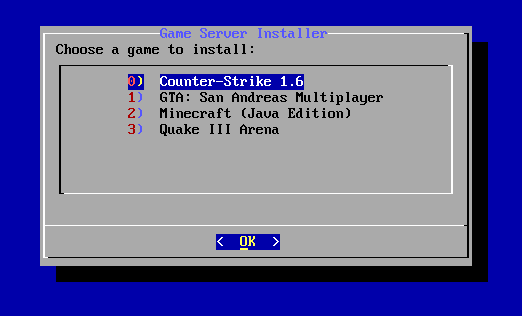
\includegraphics[width=0.7\paperwidth]{gameservers}
  \end{frame}

  \begin{frame}{Automatizace}
    Je nutné automatizovat tyto kroky:
    \begin{itemize}
      \item sestavení obrazu systému, \pause
      \item připravení obrazu pro provoz v cloudu, \pause
      \item instalace herního serveru, \pause
      \item spuštění herního serveru.
    \end{itemize}
  \end{frame}

  \begin{frame}{Zveřejnění výsledků}
    \begin{itemize}
      \item TurnKey Hub - obrazy
      \item GitHub - zdrojové kódy
    \end{itemize}
  \end{frame}

  \begin{frame}{Možnosti rozšíření}
    Všechny zdrojové kódy jsou volně dostupné, je možné:
    \begin{itemize}
      \item provozovat systém u sebe nebo v cloudu,
      \item jednoduše přidávat podporu pro nové herní servery,
      \item provozovat herní servery v komerčním prostředí.
    \end{itemize}
  \end{frame}

  \section{Shrnutí}
  \begin{frame}{Shrnutí}
    \begin{itemize}
      \item Cílem práce bylo vytvořit obraz systému pro herní servery v cloudu. 
      \item Obraz lze sestavit s využitím existujících nástrojů.
      \item Podpora až 100 různých herních serverů s možností rozšíření.
      \item Systém splňuje bezpečnostní požadavky.
      \item Celý proces je plně automatizovatelný.
    \end{itemize}
  \end{frame}

\end{document}
